%%%%%%%%%%%%%%%%%%%%%%%%%%%%%%%%%%%%%%%%%%%%%%%%%%%%%%%%%%%%%%%%%%%%%%%
%% The Legacy of Colonial Medicine in Central Africa
%% Seminar presentation (45 min) -- we present the paper as its authors
%% Template: SMILE beamer (Nasy) -- see smile_styles.tex
%%
%% Compile on Overleaf with pdfLaTeX (default). Bibliography: natbib + BibTeX.
%% Version without animations (for printing / sharing): add "handout" to
%% the class options below:  \documentclass[aspectratio=1610,handout]{beamer}
%%
%% Timing plan (30 numbered slides, target 43 min + 2 min buffer):
%%   1 Introduction                    slides  1-5    7 min
%%   2 Historical background           slides  6-9    5 min
%%   3 Data                            slides 10-11   3 min
%%   4 Empirical strategy              slides 12-15   6.5 min
%%   5 Results                         slides 16-21   9 min
%%   6 Mechanisms and policy relevance slides 22-24   4.5 min
%%   7 Discussion and conclusion       slides 25-30   8 min
%%
%% Suggested split between speakers (edit freely):
%%   Speaker 1 : sections 1-2                         (~12 min)
%%   Speaker 2 : sections 3-4 + results up to robustness, slides 10-20 (~16.5 min)
%%   Speaker 3 : slide 21 to the end                  (~14.5 min)
%%%%%%%%%%%%%%%%%%%%%%%%%%%%%%%%%%%%%%%%%%%%%%%%%%%%%%%%%%%%%%%%%%%%%%%

\documentclass[aspectratio=1610]{beamer}

\hypersetup{
  unicode,
  linkcolor=blue,
  anchorcolor=blue,
  citecolor=blue,
  filecolor=black,
  urlcolor=blue
}

%%%%% PACKAGES
\usepackage[utf8]{inputenc}
\usepackage[T1]{fontenc}
\usepackage{amsmath}
\usepackage{amssymb}
\usepackage{textcomp}
\usepackage{graphicx}
\usepackage{booktabs}
\usepackage{multirow}
\usepackage{array}
\usepackage{tikz}
\usetikzlibrary{positioning,arrows.meta}
\usepackage{appendixnumberbeamer} % backup slides are not counted in the total
\usepackage[authoryear,round]{natbib}

%%%%% STYLE (SMILE template, adapted)
%%%%%%%%%%%%%%%%%%%%%%%%%%%%%%%%%%%%%%%%%%%%%%%%%%%%%%%%%%%%%%%%%%%%%%%
%% SMILE beamer style (Nasy, https://github.com/uta-smile/beamer-theme)
%% Adapted for our seminar presentation.
%% Changes vs. the original:
%%   - footer shows presenters / short title / date / slide number
%%     instead of "Dept. CSE, UT Arlington" and the SMILE lab name;
%%   - backup slides (after \appendix) display "Backup" instead of a
%%     number, so the count shown during the talk only covers main slides;
%%   - section-outline slides are not numbered;
%%   - title page fonts, coloured blocks and a few helper colours.
%%%%%%%%%%%%%%%%%%%%%%%%%%%%%%%%%%%%%%%%%%%%%%%%%%%%%%%%%%%%%%%%%%%%%%%

\usetheme{default}
\useinnertheme{circles}
\useoutertheme{infolines}
\usefonttheme{serif}

\usepackage{etoolbox}

%% Colours
\definecolor{smileblue}{rgb}{0.2,0.2,0.7}   % beamer's default structure blue
\definecolor{accent}{rgb}{0.70,0.10,0.10}   % key numbers and warnings
\definecolor{softgray}{gray}{0.40}          % sources and citations

%% Remove navigation symbols (cleaner on a projector)
\setbeamertemplate{navigation symbols}{}

%% Frame title: title + thin rule (original SMILE style)
\setbeamertemplate{frametitle}{%
  \usebeamerfont{frametitle}\insertframetitle\strut%
  \vskip-0\baselineskip%
  \leaders\vrule width .95\paperwidth\vskip1pt%
  \vskip0pt%
  \nointerlineskip
}

%% Title page
\setbeamerfont{title}{size=\LARGE,series=\bfseries}
\setbeamerfont{author}{size=\large}
\setbeamerfont{institute}{size=\normalsize}
\setbeamerfont{date}{size=\small}
\setbeamercolor{date}{fg=softgray}

%% Blocks: used sparingly, for the research question and key take-aways
\setbeamertemplate{blocks}[rounded][shadow=false]
\setbeamercolor{block title}{fg=white,bg=smileblue}
\setbeamercolor{block body}{fg=black,bg=smileblue!7}
\setbeamercolor{block title alerted}{fg=white,bg=accent}
\setbeamercolor{block body alerted}{fg=black,bg=accent!6}
\setbeamerfont{block title}{size=\normalsize,series=\bfseries}

%% Slightly tighter nested lists
\setbeamerfont{itemize/enumerate subbody}{size=\small}
\setbeamerfont{itemize/enumerate subsubbody}{size=\footnotesize}

%% Footer
\setbeamercolor{footlinecolor}{fg=cyan,bg=green}
\setbeamercolor{author in head/foot}{fg=blue}

\newif\ifbackupslides
\backupslidesfalse
\newif\ifoutlineframe   % section-outline frames carry no slide number
\outlineframefalse

\setbeamertemplate{footline}{%
  \leavevmode%
  \hbox{%
  \begin{beamercolorbox}[wd=.26\paperwidth,ht=2.25ex,dp=1ex,left]{author in head/foot}%
    \hspace*{2ex}\usebeamerfont{author in head/foot}\insertshortauthor
  \end{beamercolorbox}%
  \begin{beamercolorbox}[wd=.50\paperwidth,ht=2.25ex,dp=1ex,center]{author in head/foot}%
    \usebeamerfont{title in head/foot}\insertshorttitle
  \end{beamercolorbox}%
  \begin{beamercolorbox}[wd=.24\paperwidth,ht=2.25ex,dp=1ex,right]{date in head/foot}%
    \usebeamerfont{date in head/foot}
    \insertshortdate{}\hspace*{1em}%
    \ifbackupslides
      Backup%
    \else
      \ifoutlineframe\else\insertframenumber/\inserttotalframenumber\fi%
    \fi
    \hspace*{2ex}
  \end{beamercolorbox}}%
  \vskip0pt%
}


\graphicspath{{figures/}}

%% Small helpers
\newcommand{\highlight}[1]{\textcolor{accent}{\textbf{#1}}}
\newcommand{\key}[1]{\textcolor{accent}{$\mathbf{#1}$}}            % key coefficient in a table
\newcommand{\refs}[1]{{\footnotesize\color{softgray}(\citealp{#1})}} % discreet citations
\newcommand{\src}[1]{{\scriptsize\color{softgray}#1}}               % source line under a table/figure
\newcommand{\backupbutton}[2]{\hyperlink{#1}{\beamergotobutton{#2}}}
\newcommand{\returnbutton}[1]{\par\vfill\hfill\hyperlink{#1}{\beamerreturnbutton{Back}}}

%% Outline at the beginning of each section (not counted in slide numbers)
\setbeamertemplate{section in toc}[sections numbered]
\AtBeginSection[]{
  {\outlineframetrue
  \begin{frame}[noframenumbering]{Outline}
    \vfill
    \tableofcontents[currentsection, hideallsubsections]
    \vfill
  \end{frame}}
}

%%%%% TITLE
%% Title slide: only our three names and the programme line.
%% Add surnames inside \author{...} if you wish, e.g. "Alexandre Dupont \and ...".
%% Replace \today by the date of the talk, e.g. \date{2 December 2026}.
\title[The Legacy of Colonial Medicine in Central Africa]%
  {The Legacy of Colonial Medicine\texorpdfstring{\\}{ }in Central Africa}
\author[Cristiano, Alexandre \& Marceau]{Cristiano Miguel \and Alexandre Fuilla-Weishaupt \and Marceau Langlais}
\institute[]{Master of Economics -- École Normale Supérieure Paris-Saclay}
\date{26 November 2026}

\begin{document}

%%%%%%%%%%%%%%%%%%%%%%%%%%%%%%%%%%%%%%%%%%%%%%%%%%%%%%%%%%%%%%%%%%%%%%%
\begin{frame}[plain,noframenumbering]
  \titlepage
\end{frame}

%%%%%%%%%%%%%%%%%%%%%%%%%%%%%%%%%%%%%%%%%%%%%%%%%%%%%%%%%%%%%%%%%%%%%%%
\section{Introduction}
%%%%%%%%%%%%%%%%%%%%%%%%%%%%%%%%%%%%%%%%%%%%%%%%%%%%%%%%%%%%%%%%%%%%%%%

\begin{frame}{A puzzle: low demand for effective health care}
  \begin{itemize}
    \item Sub-Saharan Africa carries a disproportionate share of the global disease burden
      \begin{itemize}
        \item 90\% of malaria deaths, 70\% of people living with HIV, highest under-5 mortality
      \end{itemize}
    \item Yet demand for cheap, effective preventive care remains \highlight{puzzlingly low}
      \refs{dupas_2011,banerjee_etal_2010,dupas_miguel_2017}
      \begin{itemize}
        \item An estimated 20 million children are not vaccinated \refs{who_2019};
          in our region coverage is often below herd-immunity thresholds
      \end{itemize}
    \item Usual explanations: liquidity constraints, present bias, access costs, information
    \pause
    \item \textbf{A missing piece? Mistrust of medicine}
      \begin{itemize}
        \item Ebola (West Africa 2014, DR Congo 2018--19): distrust of health workers hampered containment
          \refs{blair_etal_2017,vinck_etal_2019}
        \item Northern Nigeria: boycott of polio vaccination $\Rightarrow$ outbreak \refs{jegede_2007}
      \end{itemize}
  \end{itemize}
  \vspace{0.3em}
  \centering
  \textbf{Where does this mistrust come from?}
\end{frame}

\begin{frame}{Research question}
  \begin{block}{Research question}
    Did the colonial sleeping sickness campaigns leave a \textbf{lasting legacy of mistrust in medicine}
    that still shapes health behaviour and the success of health policy today?
  \end{block}
  \vspace{0.2em}
  \begin{columns}[T]
    \begin{column}{0.47\textwidth}
      \textbf{Three sub-questions}
      \begin{enumerate}
        \item \textbf{Behaviour:} do more exposed areas vaccinate less and refuse medical tests more?
        \item \textbf{Mechanism:} is the mistrust specific to medicine? How is it transmitted?
        \item \textbf{Policy:} do health projects work less well there today?
      \end{enumerate}
    \end{column}
    \begin{column}{0.50\textwidth}
      \textbf{What we do}
      \begin{itemize}
        \item \textbf{Setting:} French campaigns, 1921--1956, in Cameroon and former French Equatorial
          Africa (AEF): forced examinations and injections with severe side effects
        \item \textbf{Data:} 30 years of military archives, digitized and matched to today's surveys
        \item \textbf{Identification:} OLS with rich controls, an IV, and a falsification test
      \end{itemize}
    \end{column}
  \end{columns}
\end{frame}

\begin{frame}{Preview of results}
  \begin{columns}[c]
    \begin{column}{0.50\textwidth}
      \centering
      {\small Effect of 15 years of campaign visits (out of 30)}\\[0.5em]
      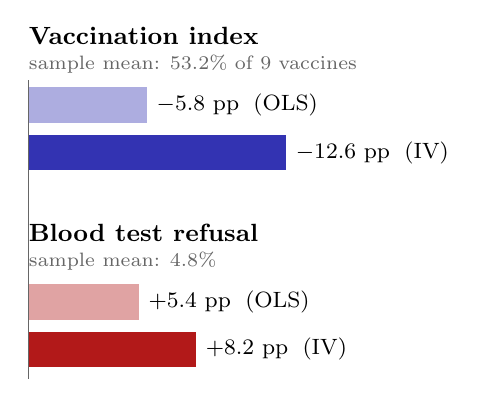
\begin{tikzpicture}[x=0.26cm,y=1cm]
        % Panel A: vaccination
        \node[anchor=west,font=\small\bfseries,inner sep=0] at (0,4.55) {Vaccination index};
        \node[anchor=west,font=\scriptsize,text=softgray,inner sep=0] at (0,4.2) {sample mean: 53.2\% of 9 vaccines};
        \fill[smileblue!40] (0,3.45) rectangle (5.8,3.9);
        \node[anchor=west,font=\footnotesize] at (5.8,3.675) {$-5.8$ pp \;(OLS)};
        \fill[smileblue] (0,2.85) rectangle (12.6,3.3);
        \node[anchor=west,font=\footnotesize] at (12.6,3.075) {$-12.6$ pp \;(IV)};
        % Panel B: refusals
        \node[anchor=west,font=\small\bfseries,inner sep=0] at (0,2.05) {Blood test refusal};
        \node[anchor=west,font=\scriptsize,text=softgray,inner sep=0] at (0,1.7) {sample mean: 4.8\%};
        \fill[accent!40] (0,0.95) rectangle (5.4,1.4);
        \node[anchor=west,font=\footnotesize] at (5.4,1.175) {$+5.4$ pp \;(OLS)};
        \fill[accent] (0,0.35) rectangle (8.2,0.8);
        \node[anchor=west,font=\footnotesize] at (8.2,0.575) {$+8.2$ pp \;(IV)};
        \draw[black!60] (0,0.2) -- (0,4.0);
      \end{tikzpicture}
    \end{column}
    \begin{column}{0.48\textwidth}
      \begin{itemize}
        \item \textbf{Vaccinations} fall by 11\% to 24\% of the mean
        \item \textbf{Refusals} of a free blood test more than double
        \item \textbf{Health-seeking:} less contact with the health system, despite \emph{equal access}
        \item \textbf{Mechanism:} mistrust is \emph{specific to medicine} and passed on mostly within ethnic groups
        \item \textbf{Policy:} World Bank \emph{health} projects rated about one notch lower;
          no effect on other sectors
      \end{itemize}
    \end{column}
  \end{columns}
\end{frame}

\begin{frame}{Related literature}
  \small
  \begin{columns}[T]
    \begin{column}{0.49\textwidth}
      \textbf{1. Historical roots of African development}\\
      Slave trades, institutions, borders, colonial investments, missions\\
      \refs{nunn_2008,nunn_2009,gennaioli_rainer_2007,huillery_2009,michalopoulos_papaioannou_2013,michalopoulos_papaioannou_2016,alsan_2015,cage_rueda_2020,anderson_2018}

      \vspace{0.45em}
      \textbf{2. Demand for health in poor countries}\\
      Prices, liquidity, present bias: mostly RCTs\\
      \refs{dupas_2011,banerjee_etal_2010,dupas_miguel_2017}

      \vspace{0.45em}
      \textbf{3. Trust: origins and consequences}\\
      Trust and development \refs{algan_cahuc_2010,nunn_wantchekon_2011}\\
      Trust and health \refs{alsan_wanamaker_2018,alsan_garrick_graziani_2019,martinez_bravo_stegmann_2022}
    \end{column}
    \begin{column}{0.49\textwidth}
      \textbf{4. Unintended effects of interventions}\\
      Aid and conflict \refs{nunn_qian_2014,crost_etal_2014,dube_naidu_2015}\\
      Historical health campaigns \refs{acemoglu_johnson_2007,kazianga_etal_2014}

      \vspace{0.7em}
      \textbf{5. History, anthropology and epidemiology of the campaigns}\\
      Archival and qualitative accounts of coercion, side effects and rumours\\
      \refs{headrick_1994,feldman_etal_2000,giles_vernick_2002,lachenal_2014,lachenal_2017}\\
      Unsafe injections and blood-borne viruses \refs{pepin_labbe_2008,pepin_2011}
    \end{column}
  \end{columns}
\end{frame}

\begin{frame}{Gaps in the literature and our contribution}
  \footnotesize
  \renewcommand{\arraystretch}{1.25}
  \begin{tabular}{@{}>{\raggedright\arraybackslash}p{0.19\textwidth}
                    >{\raggedright\arraybackslash}p{0.36\textwidth}
                    >{\raggedright\arraybackslash}p{0.37\textwidth}@{}}
    \toprule
    \textbf{Literature} & \textbf{What was missing} & \textbf{What we add} \\
    \midrule
    Colonial legacies &
      Institutions, slave trades, missions and public investments are well studied; the colonial \emph{medical campaigns} had never been studied quantitatively &
      A new archival dataset: 30 years, 5 countries, subdistrict level. First quantitative evidence on the sleeping sickness campaigns \\
    Demand for health &
      Focus on present-day constraints; the \emph{origin} of mistrust is left unexplained &
      Mistrust rooted in history as a demand-side constraint \\
    Trust and health &
      Single events, mostly in the US (Tuskegee) and short-run responses to a disclosure &
      A mass ``treatment'' of millions of people in 5 countries; persistence across generations \\
    Historians, anthropologists &
      Rich case studies and anecdotes, but no causal test &
      Causal estimates: IV and falsification test \\
    Aid effectiveness &
      No link between historical experience and today's project success &
      World Bank health projects are less successful in exposed areas \\
    \bottomrule
  \end{tabular}
\end{frame}

%%%%%%%%%%%%%%%%%%%%%%%%%%%%%%%%%%%%%%%%%%%%%%%%%%%%%%%%%%%%%%%%%%%%%%%
\section{Historical background}
%%%%%%%%%%%%%%%%%%%%%%%%%%%%%%%%%%%%%%%%%%%%%%%%%%%%%%%%%%%%%%%%%%%%%%%

\begin{frame}{Sleeping sickness and the colonial response}
  \begin{columns}[T]
    \begin{column}{0.56\textwidth}
      \begin{itemize}
        \item Lethal parasitic disease (\emph{trypanosomiasis}) transmitted by the \textbf{tsetse fly}
          \begin{itemize}
            \item Stage 1: fever, headaches, swollen lymph nodes
            \item Stage 2: nervous system, lethargy, death
          \end{itemize}
        \item Large epidemics in the early 20th century
        \item Motives for intervention: humanitarian, but also \textbf{labour supply} and scientific prestige
        \item French approach: treat the \emph{individual}\\
          (British: control the environment)
          \refs{headrick_d_2014}
      \end{itemize}
    \end{column}
    \begin{column}{0.41\textwidth}
      \centering
      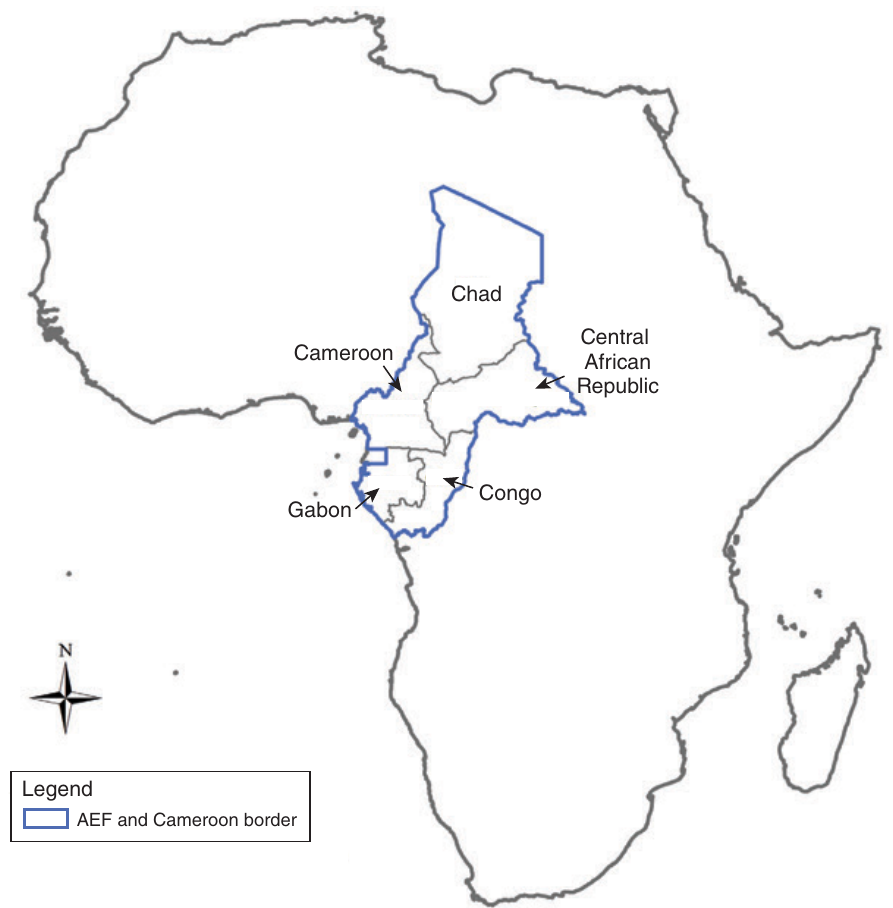
\includegraphics[height=0.62\textheight]{fig1_map}\\
      \src{Cameroon and former AEF}
    \end{column}
  \end{columns}
\end{frame}

\begin{frame}{The mobile medical teams}
  \begin{itemize}
    \item Run by the \textbf{military}: 1 French doctor, African nurses, soldiers, porters
    \item Villagers forced, often \highlight{at gunpoint}, to undergo examinations:
      neck palpation, blood tests, \textbf{lumbar punctures}
    \item Huge coverage: in Cameroon in 1928, 663{,}971 people examined, 17\% diagnosed
    \item Priority given to public health over the individual patient
  \end{itemize}
  \vspace{0.6em}
  \centering
  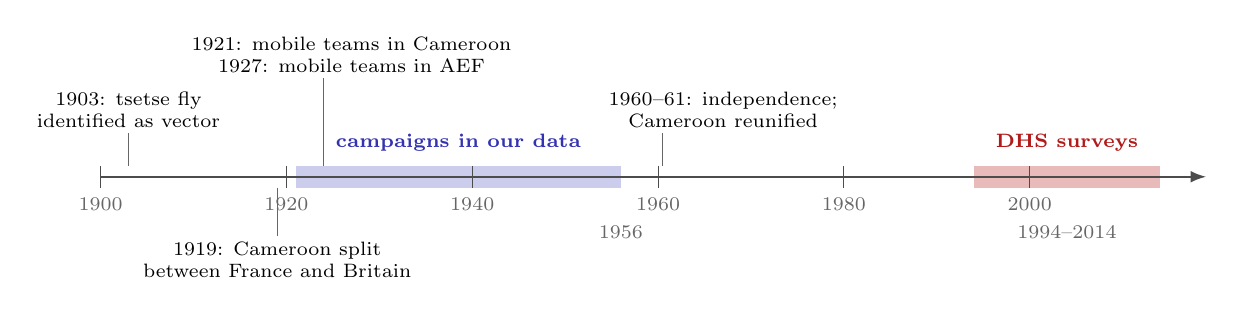
\begin{tikzpicture}[x=0.118cm,y=1cm,font=\scriptsize]
    % axis: year - 1900
    \fill[smileblue!25] (21,-0.14) rectangle (56,0.14);
    \fill[accent!30] (94,-0.14) rectangle (114,0.14);
    \draw[-{Latex[length=2mm]},thick,black!70] (0,0) -- (119,0);
    \foreach \y/\lab in {0/1900,20/1920,40/1940,60/1960,80/1980,100/2000}
      {\draw[black!70] (\y,-0.14) -- (\y,0.14); \node[below,text=softgray] at (\y,-0.14) {\lab};}
    % events above
    \draw[black!60] (3,0.14) -- (3,0.55);
    \node[above,align=center] at (3,0.5) {1903: tsetse fly\\identified as vector};
    \draw[black!60] (24,0.14) -- (24,1.25);
    \node[above,align=center] at (27,1.2) {1921: mobile teams in Cameroon\\1927: mobile teams in AEF};
    \node[above,align=center,text=smileblue] at (38.5,0.2) {\textbf{campaigns in our data}};
    \draw[black!60] (60.5,0.14) -- (60.5,0.55);
    \node[above,align=center] at (67,0.5) {1960--61: independence;\\Cameroon reunified};
    \node[above,align=center,text=accent] at (104,0.2) {\textbf{DHS surveys}};
    % events below
    \draw[black!60] (19,-0.14) -- (19,-0.75);
    \node[below,align=center] at (19,-0.7) {1919: Cameroon split\\between France and Britain};
    \node[below,align=center,text=softgray] at (104,-0.5) {1994--2014};
    \node[below,align=center,text=softgray] at (56,-0.5) {1956};
  \end{tikzpicture}
\end{frame}

\begin{frame}{The treatments: atoxyl and Lomidine}
  \begin{columns}[T]
    \begin{column}{0.48\textwidth}
      \textbf{Atoxyl} (arsenic-based)
      \begin{itemize}
        \item Therapeutic dose $\approx$ lethal dose
        \item Blindness in up to \highlight{20\%} of patients
        \item Could speed death in stage 2
        \item Used by the French until the 1930s, a decade after other colonisers stopped:
          about 7$\times$ cheaper than alternatives
      \end{itemize}
    \end{column}
    \begin{column}{0.48\textwidth}
      \textbf{Lomidine} (pentamidine)
      \begin{itemize}
        \item Mass \emph{preventive} injections for entire villages, every 6 months
        \item Pain, dizziness, gangrene, deaths
        \item Considered too dangerous for Europeans
        \item Ultimately \highlight{ineffective} as prevention
      \end{itemize}
    \end{column}
  \end{columns}
  \vspace{1em}
  \centering
  \small A French doctor involved later called the injections\\
  \emph{``pointless, dangerous, and therefore pointlessly dangerous''} \refs{lachenal_2017}
\end{frame}

\begin{frame}[label=main-memory]{The campaigns are remembered}
  \begin{itemize}
    \item Historians and anthropologists link the campaigns to mistrust of modern medicine
      \refs{headrick_1994,lachenal_2014}
    \item Cameroon, 1990: resistance to a tetanus vaccination campaign explained by
      collective memories of the sleeping sickness campaigns \refs{feldman_etal_2000}
    \item Central African Republic, late 1980s: rumours that the injections brought death
      \refs{giles_vernick_2002}
    \item The Eton (Central Cameroon) still sing about the painful injections and police violence
    \item Possible health channel too: reused needles $\Rightarrow$ spread of Hepatitis C
      \refs{pepin_2011} \backupbutton{bk-iatrogenic}{Details}
  \end{itemize}
  \vspace{0.3em}
  \begin{block}{Our hypothesis}
    Coercion + harmful side effects + ineffective drugs $\Rightarrow$ mistrust in medicine,
    \textbf{transmitted across generations}
  \end{block}
\end{frame}

%%%%%%%%%%%%%%%%%%%%%%%%%%%%%%%%%%%%%%%%%%%%%%%%%%%%%%%%%%%%%%%%%%%%%%%
\section{Data}
%%%%%%%%%%%%%%%%%%%%%%%%%%%%%%%%%%%%%%%%%%%%%%%%%%%%%%%%%%%%%%%%%%%%%%%

\begin{frame}{Historical data: the colonial medical reports}
  \begin{columns}[T]
    \begin{column}{0.57\textwidth}
      \begin{itemize}
        \item Source: \emph{Service historique de la Défense} (French military archives)
        \item Annual reports of each colony on health activities
        \item We digitized \textbf{hundreds of tables}:
          \begin{itemize}
            \item AEF: 1927--1956, subdistrict level
            \item Cameroon: 1921--1950, ethnicity-district level
          \end{itemize}
        \item Content: population, people visited, new and old cases, lumbar punctures, injections
      \end{itemize}
      \vspace{0.4em}
      \textbf{Exposure measure:}
      \[
        \text{ShareYearsVisited}_r = \frac{1}{30}\sum_{y} \text{Visited}_{y,r}
      \]
      {\small $\text{Visited}_{y,r}=1$ if region $r$ was visited in year $y$}
    \end{column}
    \begin{column}{0.40\textwidth}
      \centering
      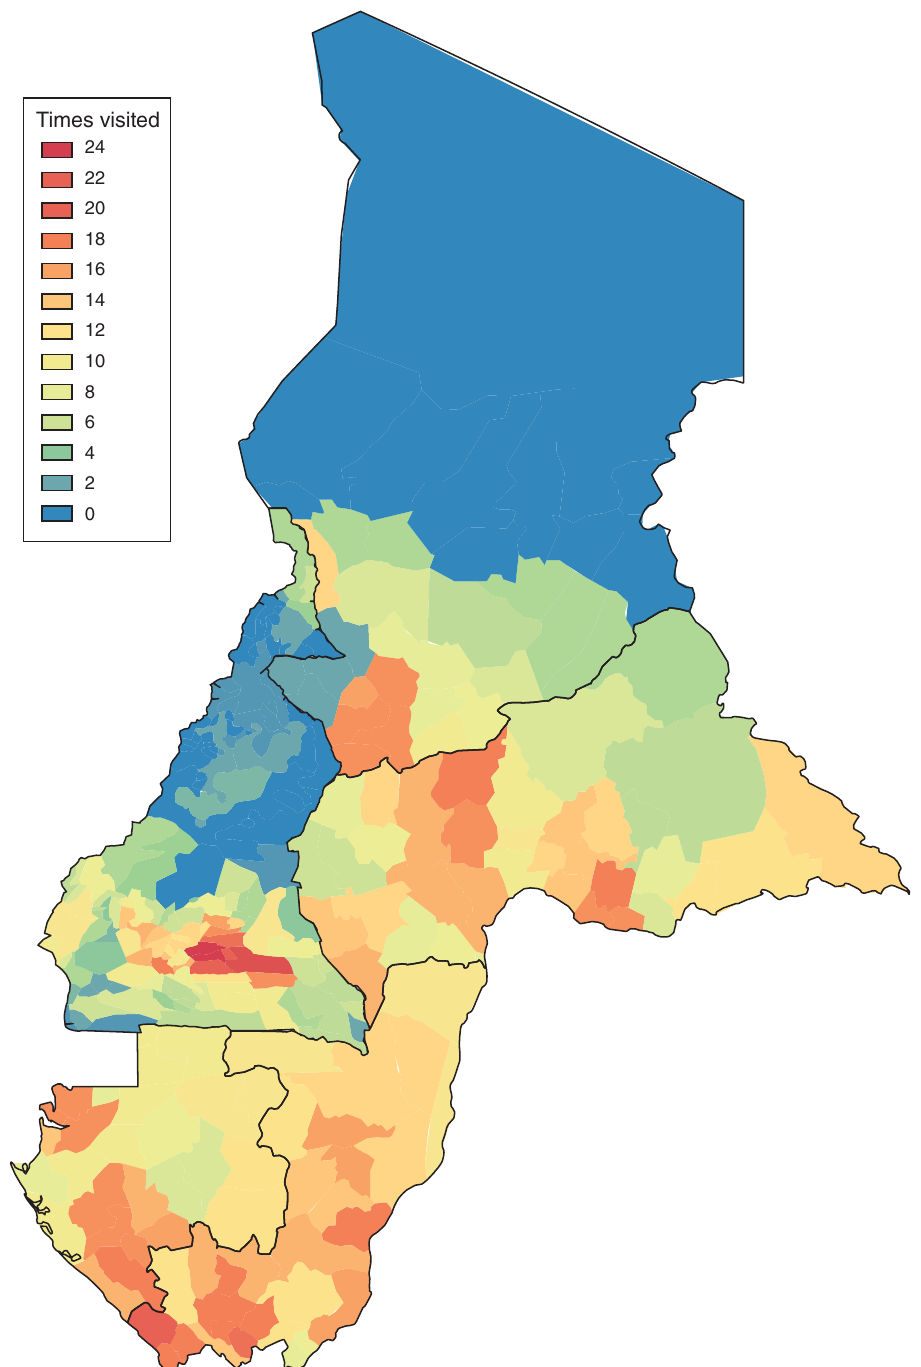
\includegraphics[height=0.70\textheight,width=\linewidth,keepaspectratio]{fig2_visits}\\
      \src{Number of years visited, 1921--1956 (0 to 24)}
    \end{column}
  \end{columns}
\end{frame}

\begin{frame}[label=main-outcomes]{Present-day data}
  \textbf{Demographic and Health Surveys (DHS)}: Cameroon (2004, 2011), Gabon (2012), Congo (2011),
  Chad (1996, 2004, 2014), CAR (1994)
  \vspace{0.3em}
  \begin{enumerate}
    \item \textbf{Vaccination index}: share of 9 vaccines completed by children under 5
      (BCG, polio 0--3, DPT 1--3, measles)
    \item \textbf{Blood test refusal}: refusing a free, non-invasive finger-prick test for
      \emph{anemia} or \emph{HIV}
      \begin{itemize}
        \item A \highlight{revealed-preference} proxy for mistrust in medicine: behaviour, not stated opinion
        \item No financial cost $\Rightarrow$ full take-up expected without mistrust
          \backupbutton{bk-interpretation}{Alternative interpretations}
      \end{itemize}
  \end{enumerate}
  \vspace{0.3em}
  \textbf{Complementary sources}
  \begin{itemize}
    \item \textbf{Afrobarometer} (Cameroon, Gabon; rounds 5--6): use of and access to health care,
      trust in people and institutions
    \item \textbf{AidData}: geolocated World Bank projects (1995--2014) and their outcome ratings
  \end{itemize}
\end{frame}

%%%%%%%%%%%%%%%%%%%%%%%%%%%%%%%%%%%%%%%%%%%%%%%%%%%%%%%%%%%%%%%%%%%%%%%
\section{Empirical strategy}
%%%%%%%%%%%%%%%%%%%%%%%%%%%%%%%%%%%%%%%%%%%%%%%%%%%%%%%%%%%%%%%%%%%%%%%

\begin{frame}{Baseline specification}
  \[
    y_{irct} = \gamma_1\, \text{ShareYearsVisited}_r + X_{irct}'\beta + X_r'\Gamma + \delta_{ct} + \varepsilon_{irct}
  \]
  \begin{itemize}
    \item $i$ individual, $r$ colonial medical report region, $c$ country, $t$ survey year
    \item $X_{irct}$: age, age$^2$, gender, urban/rural; then education and wealth fixed effects
    \item $X_r$: region-level controls
      \begin{itemize}
        \item \emph{Geography and climate}: temperature, precipitation, land suitability, altitude, area, lat./long.
        \item \emph{Disease}: malaria ecology, tsetse suitability (TSI), \textbf{initial sleeping sickness prevalence}
        \item \emph{Colonial}: Atlantic slave trade exports, Christian missions
      \end{itemize}
    \item $\delta_{ct}$: survey-year fixed effects; standard errors clustered at region $r$
    \item Also: \textbf{lasso}-selected controls \refs{belloni_chernozhukov_hansen_2014}
  \end{itemize}
  \vspace{0.2em}
  \textbf{Reading the coefficients:} $\gamma_1 \times 0.5$ = effect of being visited 15 years out of 30
\end{frame}

\begin{frame}{Threats to identification}
  \begin{enumerate}
    \item \textbf{Reverse causality / selection}
      \begin{itemize}
        \item Teams may have chosen places based on initial attitudes toward medicine
        \item OLS overstates the effect only if teams targeted \emph{less} trusting places
        \item More plausible: teams avoided resistant areas $\Rightarrow$ OLS biased \emph{toward zero}
      \end{itemize}
    \item \textbf{Omitted variables}
      \begin{itemize}
        \item Something that drives both campaign visits and attitudes today
        \item Main predictors of visits: disease suitability ($+$), rurality ($-$), missions ($-$)
          $\Rightarrow$ all controlled for
      \end{itemize}
  \end{enumerate}
  \pause
  \vspace{0.4em}
  \begin{block}{We need an instrument}
    Natural candidate: tsetse suitability index \refs{alsan_2015}. But our whole region is highly
    suitable: almost no variation $\Rightarrow$ we use it as a \emph{control} and look elsewhere
  \end{block}
\end{frame}

\begin{frame}{Instrument: suitability for cassava relative to millet}
  \[
    Z_r = \log(\text{suitability}_{\text{cassava}}) - \log(\text{suitability}_{\text{millet}})
  \]
  \centering
  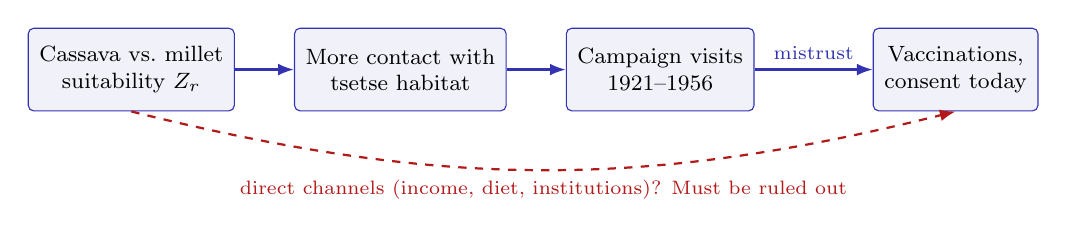
\begin{tikzpicture}[node distance=0.75cm,
      box/.style={draw=smileblue,rounded corners=2pt,align=center,font=\footnotesize,
                  inner sep=4pt,fill=smileblue!7,minimum height=1.05cm},
      arr/.style={-{Latex[length=2mm]},thick,smileblue}]
    \node[box] (Z) {Cassava vs.\ millet\\suitability $Z_r$};
    \node[box,right=of Z] (T) {More contact with\\tsetse habitat};
    \node[box,right=of T] (D) {Campaign visits\\1921--1956};
    \node[box,right=1.5cm of D] (Y) {Vaccinations,\\consent today};
    \draw[arr] (Z) -- (T);
    \draw[arr] (T) -- (D);
    \draw[arr] (D) -- node[above,font=\scriptsize,text=smileblue] {mistrust} (Y);
    \onslide<2->{
      \draw[-{Latex[length=2mm]},thick,dashed,accent] (Z.south) to[bend right=14]
        node[below,font=\scriptsize,text=accent] {direct channels (income, diet, institutions)? Must be ruled out}
        (Y.south);
    }
  \end{tikzpicture}

  \vspace{0.4em}
  \raggedright
  \textbf{Why does cassava predict campaign visits?}
  \begin{itemize}
    \item Before 1903, scientists suspected that eating cassava \emph{caused} sleeping sickness
    \item Cassava is soaked in ``cassava holes'' on river banks $\Rightarrow$ exposure to the fly
    \item 4$\times$ more calories per acre than millet $\Rightarrow$ less land cleared
      $\Rightarrow$ more tsetse-harbouring bush
  \end{itemize}
  \textbf{Why relative to millet?} To avoid capturing overall agricultural suitability
\end{frame}

\begin{frame}[label=main-relevance]{Is the instrument valid?}
  \textbf{Relevance}
  \begin{itemize}
    \item ``Zero-th stage'': $Z_r$ predicts initial sleeping sickness prevalence recorded by the teams
      \backupbutton{bk-zeroth}{Table}
    \item First stage: $Z_r$ predicts the share of years visited, $F \approx 11$ to $19$
      \backupbutton{bk-strength}{How strong?}
  \end{itemize}
  \vspace{0.5em}
  \textbf{Exclusion restriction}: $Z_r$ affects vaccinations and trust \emph{only} through the campaigns
  \begin{itemize}
    \item Concern 1: sleeping sickness itself matters for health today\\
      $\to$ we control for initial prevalence, TSI and malaria ecology
    \item Concern 2: cassava affects income, nutrition, institutions\dots\\
      $\to$ \textbf{placebo crops}: other crops relative to millet do not predict the outcomes\\
      $\to$ \textbf{falsification test}: $Z_r$ should have \emph{no} effect where there were no
      campaigns (former British Cameroon)
  \end{itemize}
\end{frame}

%%%%%%%%%%%%%%%%%%%%%%%%%%%%%%%%%%%%%%%%%%%%%%%%%%%%%%%%%%%%%%%%%%%%%%%
\section{Results}
%%%%%%%%%%%%%%%%%%%%%%%%%%%%%%%%%%%%%%%%%%%%%%%%%%%%%%%%%%%%%%%%%%%%%%%

\begin{frame}{A first look at the data}
  \centering
  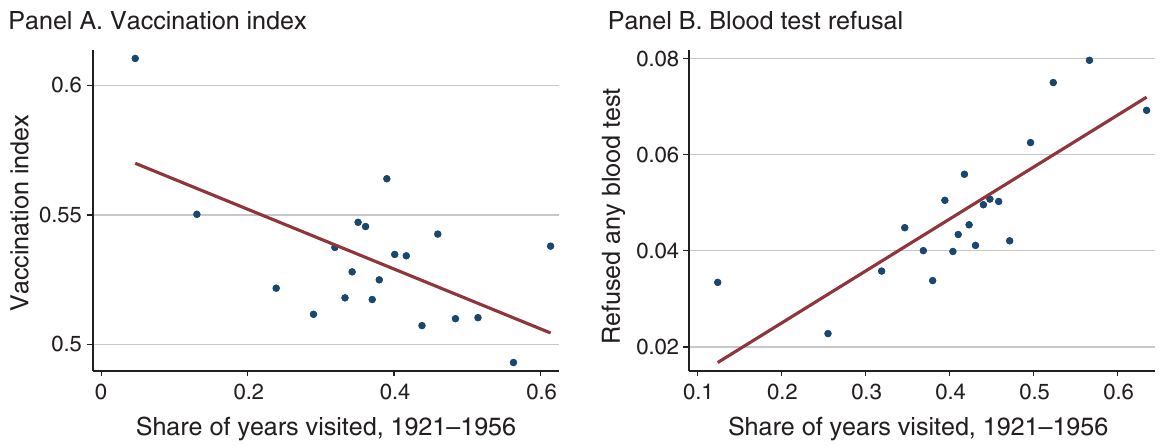
\includegraphics[width=0.90\textwidth]{fig3_binscatter}\\[0.3em]
  \src{Binned scatter plots, DHS data, residualised on baseline and contemporary controls.}

  \vspace{0.5em}
  \small
  More years of campaign visits $\Rightarrow$ \textbf{fewer} completed vaccines and \textbf{more} blood test refusals
\end{frame}

\begin{frame}[label=main-ols]{OLS estimates}
  \centering
  \small
  \begin{tabular}{lcccc}
    \toprule
    & \multicolumn{2}{c}{Vaccination index} & \multicolumn{2}{c}{Blood test refused} \\
    \cmidrule(lr){2-3}\cmidrule(lr){4-5}
    & (1) & (2) & (3) & (4) \\
    \midrule
    Share of years visited & $-0.093$ & \key{-0.116} & $0.128$ & \key{0.108} \\
                           & (0.047)  & (0.044)  & (0.035) & (0.028) \\
    \midrule
    Baseline controls      & Yes & Yes & Yes & Yes \\
    Contemporary controls  & No  & Yes & No  & Yes \\
    Observations           & 50,773 & 50,668 & 71,052 & 71,001 \\
    Clusters               & 207 & 207 & 160 & 160 \\
    Mean dep.\ var.        & 0.532 & 0.532 & 0.048 & 0.048 \\
    \bottomrule
  \end{tabular}

  \pause
  \vspace{0.6em}
  \raggedright
  \begin{itemize}
    \item 15 years visited $\Rightarrow$ vaccination index \highlight{$-5.8$ pp}:
      about half a vaccine out of nine
    \item 15 years visited $\Rightarrow$ refusals \highlight{$+5.4$ pp}: from 4.8\% to about 10\%
    \item Stable when adding education and wealth, or with lasso-selected controls
      \backupbutton{bk-ols}{Full table}
  \end{itemize}
\end{frame}

\begin{frame}[label=main-iv]{IV estimates}
  \centering
  \small
  \begin{tabular}{lcccc}
    \toprule
    & \multicolumn{2}{c}{Vaccination index} & \multicolumn{2}{c}{Blood test refused} \\
    \cmidrule(lr){2-3}\cmidrule(lr){4-5}
    & (1) & (2) & (3) & (4) \\
    \midrule
    \multicolumn{5}{l}{\emph{Second stage (2SLS)}} \\
    Share of years visited & $-0.082$ & \key{-0.251} & $0.201$ & \key{0.164} \\
                           & (0.149)  & (0.148)  & (0.068) & (0.059) \\
    \midrule
    \multicolumn{5}{l}{\emph{First stage}} \\
    Cassava vs.\ millet    & $0.061$ & $0.060$ & $0.085$ & $0.084$ \\
                           & (0.018) & (0.018) & (0.020) & (0.019) \\
    $F$-stat (excluded instrument) & 11.3 & 11.4 & 18.9 & 19.5 \\
    \midrule
    Contemporary controls  & No & Yes & No & Yes \\
    \bottomrule
  \end{tabular}

  \pause
  \vspace{0.4em}
  \raggedright
  \begin{itemize}
    \item 15 years visited $\Rightarrow$ vaccination index \highlight{$-12.6$ pp}, refusals \highlight{$+8.2$ pp}
    \item Refusals: precisely estimated. Vaccinations: larger but imprecise ($p \approx 0.09$ in column 2)
    \item IV larger than OLS in magnitude: consistent with teams \emph{avoiding} resistant areas
      \backupbutton{bk-ivols}{Other readings} \backupbutton{bk-iv}{Full table}
  \end{itemize}
\end{frame}

\begin{frame}[label=main-falsif]{Falsification test: former British vs.\ French Cameroon}
  \begin{columns}[c]
    \begin{column}{0.31\textwidth}
      \centering
      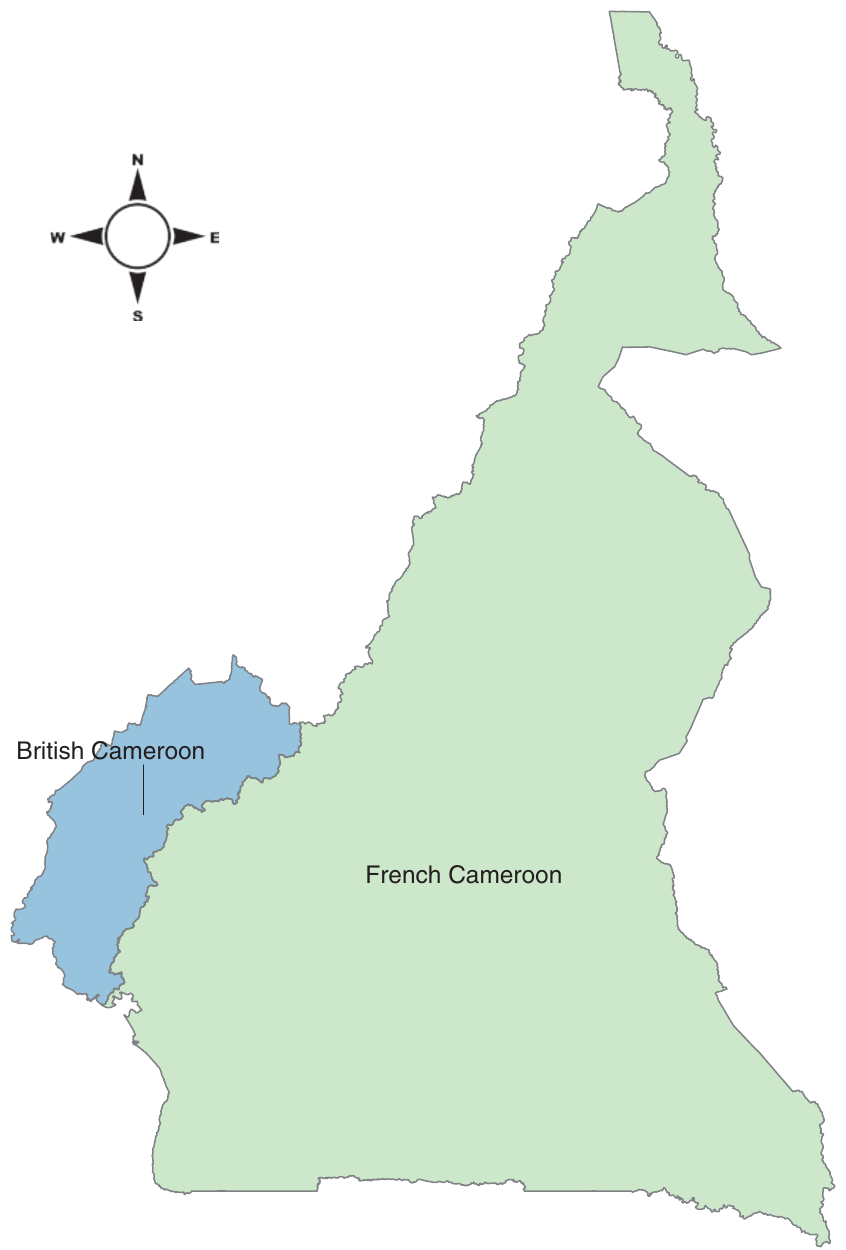
\includegraphics[height=0.66\textheight]{fig4_cameroon}
    \end{column}
    \begin{column}{0.66\textwidth}
      \begin{itemize}
        \item Cameroon split after WWI; the British ran \textbf{no campaigns} (``benign neglect'')
        \item Reunified in 1961 $\Rightarrow$ same national institutions today
        \item Reduced form of $Z_r$ within \textbf{50 km} of the old border \refs{dupraz_2019}
      \end{itemize}
      \vspace{0.3em}
      \centering
      \footnotesize
      \begin{tabular}{@{}lccc@{}}
        \toprule
        Effect of $Z_r$ on: & British side & French side & $p$-value (equal) \\
        \midrule
        Vaccination index  & $0.0045$ & \key{-0.0111} & 0.017 \\
                           & (0.0045) & (0.0047)      &       \\
        Blood test refused & $-0.0018$ & \key{0.0067} & 0.057 \\
                           & (0.0032)  & (0.0031)     &       \\
        \bottomrule
      \end{tabular}

      \pause
      \vspace{0.5em}
      \raggedright\small
      $\Rightarrow$ The instrument predicts outcomes \textbf{only} where campaigns took place:
      no sign of a direct effect of cassava suitability
      \backupbutton{bk-falsification}{More}
    \end{column}
  \end{columns}
\end{frame}

\begin{frame}[label=main-robust]{Other robustness checks}
  Results hold when:
  \begin{itemize}
    \item adding control sets one at a time, or selecting them by \textbf{lasso}
    \item using \textbf{anemia} tests only or \textbf{HIV} tests only
      $\Rightarrow$ not driven by fear of an HIV result
    \item adding \textbf{pre-colonial} ethnic controls (centralisation, plough, slavery, agriculture)
    \item controlling for sleeping sickness prevalence at several dates
    \item including Northern Chad (never visited, unsuitable for tsetse)
    \item using \textbf{WHO} vaccination data instead of DHS
    \item running the falsification test on British and Portuguese colonies vs.\ AEF:
      coefficient 8 to 10 times smaller outside the French colonies
  \end{itemize}
  \backupbutton{bk-robust}{Details}
\end{frame}

\begin{frame}{Less use of health care, despite equal access}
  \begin{columns}[c]
    \begin{column}{0.55\textwidth}
      \centering
      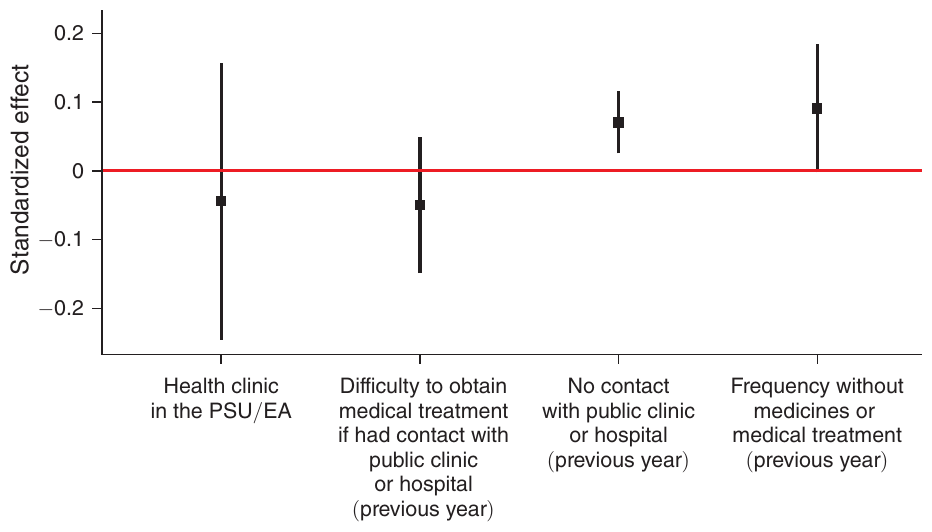
\includegraphics[width=\textwidth]{fig5_afrobarometer}\\
      \src{Standardised OLS effects of share of years visited, Afrobarometer (Cameroon, Gabon)}
    \end{column}
    \begin{column}{0.42\textwidth}
      \begin{itemize}
        \item \textbf{No difference} in having a health clinic nearby
        \item \textbf{No difference} in difficulty of getting treatment (if contact)
        \item But in more exposed areas, people:
          \begin{itemize}
            \item more often have \emph{no contact} with public clinics
            \item more often go \emph{without treatment}
          \end{itemize}
        \item[$\Rightarrow$] A \highlight{demand-side} effect, not a supply-side one
      \end{itemize}
    \end{column}
  \end{columns}
\end{frame}

%%%%%%%%%%%%%%%%%%%%%%%%%%%%%%%%%%%%%%%%%%%%%%%%%%%%%%%%%%%%%%%%%%%%%%%
\section{Mechanisms and policy relevance}
%%%%%%%%%%%%%%%%%%%%%%%%%%%%%%%%%%%%%%%%%%%%%%%%%%%%%%%%%%%%%%%%%%%%%%%
\begin{frame}[label=main-wb]{Do health projects work less well today?}
  \begin{center}
    \small
    Examining World Bank funded projects between 1995 and 2014 (AidData) rated on a six-point scale ranging from highly unsatisfactory to highly satisfactory
  \end{center}
  \vspace{0.5em}
  \centering
  \small
  \begin{tabular}{lccc}
    \toprule
    World Bank project rating  & (1) & (2) & (3) \\
    \midrule
    Health project $\times$ share of years visited & \key{-2.090} & \key{-2.100} & \key{-1.979} \\
                                                   & (0.662) & (0.668) & (0.640) \\
    \midrule
    Controls & Geography & All & All + Lasso \\
    \bottomrule
  \end{tabular}\\[0.2em]
  \src{OLS estimation on Health project × share of years visited with country and country-by-health-project
fixed effects.}

  \vspace{0.5em}
  \raggedright
  \begin{itemize}
    \item At mean exposure: a health project falls from \emph{moderately satisfactory} to
      \emph{moderately unsatisfactory}
    \item \textbf{No} negative effect on non-health projects
    \item Campaigns do not predict where projects go or which ones are rated (no selection bias)
      \backupbutton{bk-wb}{Selection checks}
  \end{itemize}
\end{frame}

\begin{frame}{Is the mistrust specific to medicine?}
  \begin{itemize}
    \item Afrobarometer trust questions (Cameroon, Gabon)
      \begin{itemize}
        \item Round 5: neighbours, parents, people you know, most people
        \item Round 6: president, parliament, local government, police, courts, traditional and religious leaders\dots
      \end{itemize}
    \item Average effect size (AES) across questions:
  \end{itemize}
  \centering
  \small
  \begin{tabular}{lcccc}
    \toprule
    & \multicolumn{2}{c}{Round 5 (people)} & \multicolumn{2}{c}{Round 6 (institutions)} \\
    \cmidrule(lr){2-3}\cmidrule(lr){4-5}
    Share of years visited & $-0.010$ & $-0.006$ & $0.003$ & $0.003$ \\
                           & (0.009)  & (0.009)  & (0.006) & (0.006) \\
    Contemporary controls  & No & Yes & No & Yes \\
    \bottomrule
  \end{tabular}

  \vspace{0.6em}
  \raggedright
  $\Rightarrow$ Coefficients are small and insignificant: the mistrust is \highlight{specific to the medical domain}
\end{frame}

\begin{frame}[label=main-transmission]{How is mistrust transmitted?}
  \begin{itemize}
    \item Data from Cameroon DHS 2004
    \item \textbf{Vertical} (parents $\to$ children) : exposure of the individual's own ethnic group vs.\ \textbf{Horizontal} (peers) : exposure of the \emph{other} ethnic groups present in the same DHS cluster
  \end{itemize}

  \vspace{0.3em}
  \centering
  \footnotesize
  \setlength{\tabcolsep}{4pt}
  \begin{tabular}{lccc}
    \toprule
    Blood test refused & (1) & (2) & (3) \\
    \midrule
    Own ethnic group's exposure          & $0.088$ & $0.074$ & $0.096$ \\
                                         & (0.035) & (0.032) & (0.034) \\
    Other ethnic groups in same location & --      & $0.033$ & $0.064$ \\
                                         &         & (0.041) & (0.034) \\
    \midrule
    Controls & Geography & All & All + Lasso \\
    \bottomrule
  \end{tabular}

  \vspace{0.4em}
  \raggedright
  \begin{itemize}
    \item Effect of exposure to colonial medical campaigns is driven by the exposure of an individual's \textbf{own ethnic group} (effect is \textbf{twice as large}) $\Rightarrow$ consistent with vertical transmission
    \item {Suggestive only: the two coefficients are not statistically different} \backupbutton{bk-transmission}{Full table}
  \end{itemize}
\end{frame}

%%%%%%%%%%%%%%%%%%%%%%%%%%%%%%%%%%%%%%%%%%%%%%%%%%%%%%%%%%%%%%%%%%%%%%%
\section{Discussion and conclusion}
%%%%%%%%%%%%%%%%%%%%%%%%%%%%%%%%%%%%%%%%%%%%%%%%%%%%%%%%%%%%%%%%%%%%%%%

\begin{frame}{Strengths of the paper}
  \begin{itemize}
    \item \textbf{New data:} 30 years of archives digitized for 5 countries, at a fine geographic level
      \begin{itemize}
        \item A public good for economists, historians and epidemiologists
      \end{itemize}
    \item \textbf{Behaviour, not opinions:} consent to a real blood test and actual vaccinations
    \item \textbf{Triangulation of identification:} OLS with rich controls and lasso, IV,
      within-country falsification test, placebo crops, placebo outcomes (other forms of trust)
    \item \textbf{Three independent data sources} point the same way:
      DHS, Afrobarometer, World Bank ratings
    \item \textbf{From history to policy:} we go beyond persistence and show consequences for
      today's health projects
    \item \textbf{A mechanism, not only a correlation:} medicine-specific mistrust, with equal access to care
  \end{itemize}
\end{frame}

\begin{frame}{Limitations : measurement and data quality}
  \begin{itemize}
    \item \textbf{Archives written by the coloniser:} military reports with their own reporting
      incentives; different units across colonies (ethnicity-district vs.\ subdistrict)
    \item \textbf{Coarse exposure measure:} share of years visited
      \begin{itemize}
        \item Not the number of injections, the drug used, or the degree of coercion and harm
      \end{itemize}
    \item \textbf{Trust is proxied:} no survey question on trust in medicine
      \begin{itemize}
        \item Only 4.8\% refuse; refusal may also reflect fear of results, stigma or the survey team
      \end{itemize}
    \item \textbf{Vaccination:} supply is not observed in the DHS; evidence of equal access comes from
      two countries only
    \item \textbf{Heterogeneous surveys:} from 1994 to 2014; district-level matching for Congo and part of
      Chad; no biomarkers in CAR
    \item \textbf{Small samples for secondary results:} 215 projects in 72 clusters; 25 ethnic groups
  \end{itemize}
\end{frame}

\begin{frame}{Beyond the paper: related evidence and open questions}
  \small
      \textbf{The same pattern elsewhere}
      \begin{itemize}
        \item \textbf{US:} Tuskegee disclosure reduced Black men's use of health care
          \refs{alsan_wanamaker_2018}
        \item \textbf{Pakistan:} after the CIA's fake vaccination campaign, immunisation fell by 23--39\%
          in districts with high Islamist support \refs{martinez_bravo_stegmann_2022}
        \item \textbf{Nigeria:} after the Pfizer trial scandal, Muslim mothers vaccinated less
          \refs{archibong_annan_2021}
        \item \textbf{Africa-wide:} mistrust and the slave trade predict lower vaccination
          \refs{stoop_etal_2021,athias_macina_2022}
      \end{itemize}
\end{frame}

\begin{frame}{Conclusion}
  \begin{enumerate}
    \item Greater exposure to colonial campaigns $\Rightarrow$ \textbf{fewer vaccinations} and \textbf{more refusals}
      of free blood tests today
    \item The effect is \textbf{specific to medicine}, transmitted within and between ethnic groups, and it weakens
      present-day \textbf{health policy}
  \end{enumerate}
  \vspace{0.6em}
  \begin{block}{Take-aways for policy}
    \begin{itemize}
      \item History matters for the design of development interventions, as coercive health campaigns have long-term effects that can persist across generetions
      \item Building demand for health care may first require \highlight{rebuilding trust in medicine}
    \end{itemize}
  \end{block}
\end{frame}

%%%%%%%%%%%%%%%%%%%%%%%%%%%%%%%%%%%%%%%%%%%%%%%%%%%%%%%%%%%%%%%%%%%%%%%
%% BACKUP SLIDES -- not counted in the slide total
%%%%%%%%%%%%%%%%%%%%%%%%%%%%%%%%%%%%%%%%%%%%%%%%%%%%%%%%%%%%%%%%%%%%%%%
\appendix
\backupslidestrue

\begin{frame}[plain]
  \centering
  \vfill
  {\Huge Backup slides}
  \vfill
\end{frame}

\begin{frame}[label=bk-interpretation]{Interpreting blood test refusal}
  \begin{itemize}
    \item \textbf{Our reading:} refusal of a free test reveals mistrust of medicine
    \item \textbf{Alternative costs of the test}
      \begin{itemize}
        \item Medical risk and discomfort of a finger prick $\Rightarrow$ should not vary across regions
        \item Fear of learning one's status $\Rightarrow$ much lower for anemia than for HIV;
          results hold for \emph{each} test separately
        \item HIV test is anonymous: no result given (but a voluntary testing team follows up)
      \end{itemize}
    \item The DHS has no survey question on trust in medicine; CAR collects no biomarkers
  \end{itemize}
  \returnbutton{main-outcomes}
\end{frame}

\begin{frame}[label=bk-ols]{OLS estimates: full table}
  \centering
  \footnotesize
  \begin{tabular}{lcccccc}
    \toprule
    & \multicolumn{3}{c}{Vaccination index} & \multicolumn{3}{c}{Blood test refused} \\
    \cmidrule(lr){2-4}\cmidrule(lr){5-7}
    & (1) & (2) & (3) & (4) & (5) & (6) \\
    \midrule
    Share of years visited & $-0.093$ & $-0.116$ & $-0.116$ & $0.128$ & $0.108$ & $0.115$ \\
                           & (0.047)  & (0.044)  & (0.044)  & (0.035) & (0.028) & (0.029) \\
    \midrule
    Geography \& climate   & Yes & Yes & Yes & Yes & Yes & Yes \\
    Disease suitability    & Yes & Yes & Yes & Yes & Yes & Yes \\
    Colonial               & Yes & Yes & Yes & Yes & Yes & Yes \\
    Contemporary           & No  & Yes & Yes & No  & Yes & Yes \\
    Lasso-selected         & No  & No  & Yes & No  & No  & Yes \\
    Observations & 50,773 & 50,668 & 50,668 & 71,052 & 71,001 & 71,001 \\
    Clusters     & 207 & 207 & 207 & 160 & 160 & 160 \\
    Mean dep.\ var. & 0.532 & 0.532 & 0.532 & 0.048 & 0.048 & 0.048 \\
    \bottomrule
  \end{tabular}

  \vspace{0.5em}
  \raggedright\scriptsize
  SE clustered at the ethnic group-district (Cameroon), colonial subdistrict (Gabon, CAR, Chad 2014)
  or district level (Congo, Chad 1996/2004). All regressions include age, age$^2$, gender, urban/rural
  and survey-year fixed effects.
  \returnbutton{main-ols}
\end{frame}

\begin{frame}[label=bk-iv]{IV estimates: full table}
  \centering
  \footnotesize
  \begin{tabular}{lcccccc}
    \toprule
    & \multicolumn{3}{c}{Vaccination index} & \multicolumn{3}{c}{Blood test refused} \\
    \cmidrule(lr){2-4}\cmidrule(lr){5-7}
    & (1) & (2) & (3) & (4) & (5) & (6) \\
    \midrule
    \multicolumn{7}{l}{\emph{Panel A. First stage (dep.\ var.: share of years visited)}} \\
    Cassava vs.\ millet & $0.061$ & $0.060$ & $0.038$ & $0.085$ & $0.084$ & $0.047$ \\
                        & (0.018) & (0.018) & (0.016) & (0.020) & (0.019) & (0.017) \\
    $F$-stat            & 11.26 & 11.38 & -- & 18.89 & 19.45 & -- \\
    Mean dep.\ var.     & 0.372 & 0.372 & 0.372 & 0.416 & 0.416 & 0.416 \\
    \midrule
    \multicolumn{7}{l}{\emph{Panel B. Second stage (2SLS)}} \\
    Share of years visited & $-0.082$ & $-0.251$ & $-0.297$ & $0.201$ & $0.164$ & $0.271$ \\
                           & (0.149)  & (0.148)  & (0.167)  & (0.068) & (0.059) & (0.064) \\
    \midrule
    Contemporary   & No & Yes & Yes & No & Yes & Yes \\
    Lasso-selected & No & No  & Yes & No & No  & Yes \\
    Observations & 50,773 & 50,668 & 50,668 & 71,052 & 71,001 & 71,001 \\
    Clusters     & 207 & 207 & 207 & 160 & 160 & 160 \\
    \bottomrule
  \end{tabular}
  \returnbutton{main-iv}
\end{frame}

\begin{frame}[label=bk-ivols]{Why is the IV estimate larger than OLS?}
  \begin{itemize}
    \item \textbf{Our preferred reading: negative selection.}
      Teams avoided areas that resisted them, so the most mistrustful places were visited \emph{less}
      $\Rightarrow$ OLS understates the effect
    \item \textbf{Measurement error.} Share of years visited is a noisy measure of true exposure
      (archival gaps, aggregation to districts) $\Rightarrow$ attenuation in OLS, corrected by IV
    \item \textbf{Local average treatment effect.} IV identifies the effect for regions whose
      exposure responds to cassava suitability, which may be those where campaigns were most intense
    \item \textbf{A violation of the exclusion restriction} would also inflate IV:
      this is why the falsification test matters
  \end{itemize}
  \vspace{0.4em}
  \textbf{Magnitudes:} our benchmark is 15 years (share $=0.5$). In the estimation samples the mean share
  is 0.37 to 0.42 (11 to 12.5 years): at those means, OLS gives $-4.3$ pp for vaccinations and $+4.5$ pp
  for refusals
  \returnbutton{main-iv}
\end{frame}

\begin{frame}[label=bk-strength]{How strong is the instrument?}
  \begin{itemize}
    \item First-stage $F$: 11.3 to 11.4 (vaccination sample), 18.9 to 19.5 (blood test sample)
    \item Above the usual rule of thumb of 10
    \item But recent work shows that the standard 5\% $t$-test is only fully reliable for
      $F > 104.7$; below, confidence intervals should be widened \refs{lee_etal_2022}
    \item What this means for us:
      \begin{itemize}
        \item Blood test refusals: $t \approx 2.8$ to $3.0$, the more robust result
        \item Vaccination index: $t \approx 1.7$ to $1.8$ at best, so the IV mainly confirms the sign
          and the order of magnitude of the OLS estimate
      \end{itemize}
    \item The reduced form (instrument on outcomes) does not suffer from weak-instrument bias:
      this is what the Cameroon border test uses
  \end{itemize}
  \returnbutton{main-relevance}
\end{frame}

\begin{frame}[label=bk-zeroth]{``Zero-th'' stage: instrument and initial prevalence}
  \centering
  \footnotesize
  \begin{tabular}{lccccc}
    \toprule
    Initial sleeping sickness prevalence & (1) & (2) & (3) & (4) & (5) \\
    \midrule
    Cassava vs.\ millet & $0.023$ & $0.027$ & $0.030$ & $0.031$ & $0.031$ \\
                        & (0.008) & (0.008) & (0.009) & (0.009) & (0.009) \\
    \midrule
    Geography \& climate & No & Yes & Yes & Yes & Yes \\
    Disease suitability  & No & No  & Yes & Yes & Yes \\
    Colonial             & No & No  & No  & Yes & Yes \\
    Lasso-selected       & No & No  & No  & No  & Yes \\
    Observations & 347 & 347 & 347 & 347 & 347 \\
    Mean dep.\ var. & 0.044 & 0.044 & 0.044 & 0.044 & 0.044 \\
    \bottomrule
  \end{tabular}

  \vspace{0.5em}
  \raggedright\small
  The instrument also predicts sleeping sickness across sub-Saharan ethnic groups (tsetse-based
  estimates from the 1970s). Because prevalence could matter directly, we control for initial prevalence.
  \returnbutton{main-relevance}
\end{frame}

\begin{frame}[label=bk-falsification]{Falsification tests: details}
  \centering
  \footnotesize
  \begin{tabular}{lcccc}
    \toprule
    & \multicolumn{2}{c}{Vaccination index} & \multicolumn{2}{c}{Blood test refused} \\
    \cmidrule(lr){2-3}\cmidrule(lr){4-5}
    & British & French & British & French \\
    \midrule
    Cassava vs.\ millet (no contemp.) & $0.0044$ & $-0.0104$ & $-0.0016$ & $0.0062$ \\
                                      & (0.0046) & (0.0053)  & (0.0033)  & (0.0031) \\
    Cassava vs.\ millet (contemp.)    & $0.0045$ & $-0.0111$ & $-0.0018$ & $0.0067$ \\
                                      & (0.0045) & (0.0047)  & (0.0032)  & (0.0031) \\
    $p$-value British = French        & -- & 0.035 / 0.017 & -- & 0.083 / 0.057 \\
    Observations & 2,019 & 3,605 & 4,867 & 7,891 \\
    Mean dep.\ var. & 0.774 & 0.743 & 0.028 & 0.062 \\
    \bottomrule
  \end{tabular}

  \vspace{0.5em}
  \raggedright\small
  \begin{itemize}
    \item Same results with 75 km and 100 km bandwidths
    \item Instrument does not predict assets or school enrolment at the border
    \item British and Portuguese colonies vs.\ AEF: coefficient effectively zero, 8--10$\times$ smaller
  \end{itemize}
  \returnbutton{main-falsif}
\end{frame}

\begin{frame}[label=bk-robust]{Robustness: details}
  \begin{itemize}
    \item Sequential addition of control groups: coefficients stable
    \item Anemia-only and HIV-only refusals: same sign and magnitude
    \item Pre-colonial controls \citep[Murdock's Ethnographic Atlas;][]{nunn_wantchekon_2011}:
      political centralisation, plough use, indigenous slavery, agriculture
    \item Sleeping sickness prevalence: first measure, average over the first 3 visits, maximum ever recorded
    \item Northern Chad included (desert, never visited)
    \item WHO vaccination coverage data
    \item Placebo instruments: other crops relative to millet do not predict outcomes
  \end{itemize}
  \returnbutton{main-robust}
\end{frame}

\begin{frame}[label=bk-transmission]{Transmission: full table}
  \centering
  \footnotesize
  \begin{tabular}{lccccc}
    \toprule
    Blood test refused & (1) & (2) & (3) & (4) & (5) \\
    \midrule
    Own ethnic group's exposure & $0.088$ & $0.086$ & $0.091$ & $0.074$ & $0.096$ \\
                                & (0.035) & (0.037) & (0.037) & (0.032) & (0.035) \\
                                & [0.130] & [0.156] & [0.146] & [0.116] & [0.094] \\
    Other ethnic groups, same location & -- & $0.030$ & $0.047$ & $0.033$ & $0.064$ \\
                                &         & (0.040) & (0.043) & (0.041) & (0.034) \\
                                &         & [0.406] & [0.240] & [0.374] & [0.072] \\
    \midrule
    Geography \& climate & Yes & Yes & Yes & Yes & Yes \\
    Disease suitability  & No  & No  & Yes & Yes & Yes \\
    Colonial, contemporary & No & No & No & Yes & Yes \\
    Lasso-selected       & No  & No  & No  & No  & Yes \\
    Observations & 8,239 & 7,189 & 7,189 & 7,189 & 7,189 \\
    Clusters (ethnic groups) & 25 & 25 & 25 & 25 & 25 \\
    Mean dep.\ var. & 0.113 & 0.119 & 0.119 & 0.119 & 0.119 \\
    \bottomrule
  \end{tabular}

  \vspace{0.4em}
  \raggedright\scriptsize
  Cameroon DHS 2004. Standard errors clustered by ethnic group in parentheses; wild-bootstrap
  $p$-values (1,000 draws) in brackets.
  \returnbutton{main-transmission}
\end{frame}

\begin{frame}[label=bk-wb]{World Bank projects: selection checks}
  \begin{itemize}
    \item Concern: campaigns could affect \emph{where} projects go or \emph{which} get rated
    \item Exposure to the campaigns does \textbf{not} predict:
      \begin{itemize}
        \item receiving any World Bank project
        \item receiving a health project
        \item a project receiving a rating
      \end{itemize}
    \item Coefficients effectively zero in all specifications
    \item Remaining limitation: we compare projects \emph{conditional on being present}
  \end{itemize}
  \returnbutton{main-wb}
\end{frame}

\begin{frame}[label=bk-iatrogenic]{A health channel: iatrogenic disease}
  \begin{itemize}
    \item Reused, unsterilised needles may have spread blood-borne viruses \refs{pepin_labbe_2008}
    \item Cameroon has one of the highest Hepatitis C rates in the world;
      HCV is linked to exposure to the campaigns
    \item Similar evidence for HTLV-1 in former AEF
    \item The campaigns may have helped the early spread of HIV \refs{pepin_2011}
    \item Comparable case: anti-schistosomiasis campaigns and HCV in Egypt
  \end{itemize}
  \returnbutton{main-memory}
\end{frame}

\begin{frame}[allowframebreaks]{References}
  \scriptsize
  \bibliographystyle{plainnat}
  \bibliography{references}
\end{frame}

\end{document}
